% one-figure manuscript written by fig_qc.py --tek-sekil-tex (trap T29)
\begin{figure*}[!t]
\centering
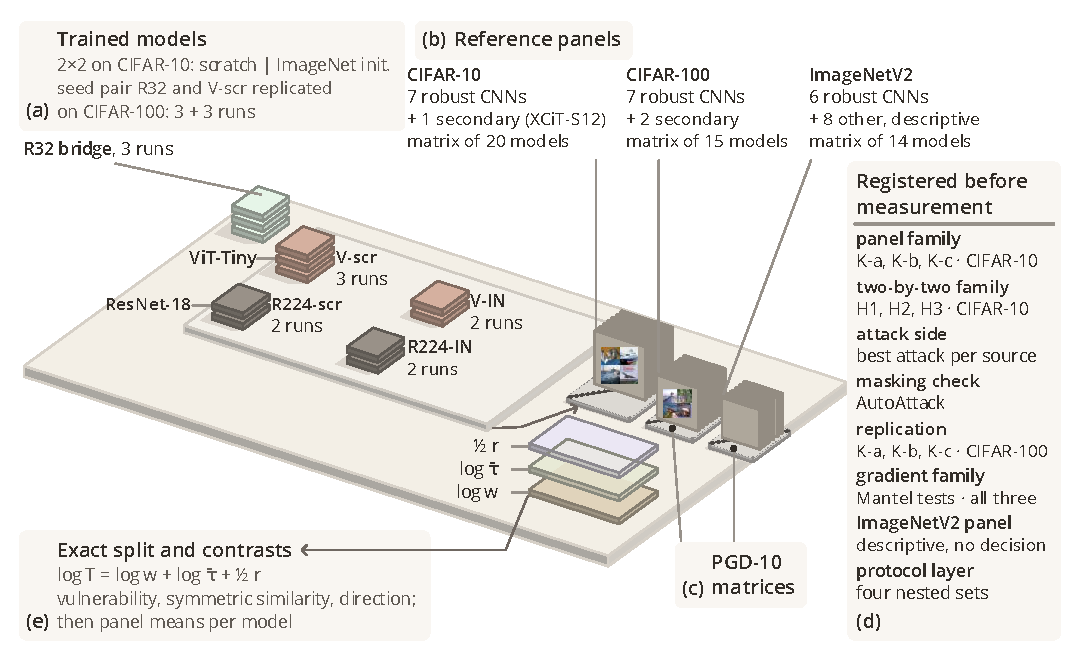
\includegraphics{fig1_study_overview}
\caption{\textbf{Study overview as one scene.} (a) Trained models: the two-by-two design, one slice per run, beside the R32 bridge; (b) Reference panels, decks of robust CNNs, sliced into (c) their PGD-10 matrices; (d) Registered before measurement gives the test families; (e) Exact split and contrasts factors each log rate. Depth runs from inputs (back) to the derived split (front).}
\label{fig:fig1_study_overview}
\end{figure*}
